\documentclass[svgnames,11pt]{beamer}
\setbeamercolor{structure}{fg=SlateGray}
\usetheme{Goettingen}
\input{/home/tof/Documents/Cozy/latex-include/preambule_commun.tex}
%\usepackage{pgfpages}
%\setbeameroption{show notes on second screen=left}
\author[]{Christophe Viroulaud}
\title{Principe du routage}
\date{}
%\logo{}
%\institute{Seconde SNT}
%\institute{Première NSI}
\institute{Terminale NSI}
\setbeamertemplate{navigation symbols}{}
\setbeamertemplate{footline}[frame number]

\begin{document}
\begin{frame}
\titlepage
\end{frame}

\section{Problématique}
\begin{frame}
    \frametitle{Juin 2020 1,78 milliards de sites web}

    
\begin{center}
    \framebox{Comment retrouver une machine précise dans le réseau?}
\end{center}

\end{frame}

\section{Adresse IP}
\begin{frame}
    \frametitle{adresse IPv4}

    \begin{center}
        \large{192.168.10.3}
    \end{center}

\end{frame}
\begin{frame}
    \frametitle{Masque de sous-réseau}

    \begin{center}
        \begin{tabular}{ccccc}
            adresse IP & 192 & 168 & 10  & 3 \\
            masque     & 255 & 255 & 255 & 0 \\
        \end{tabular}
    \end{center}

\end{frame}

\begin{frame}
    \frametitle{Porte logique AND}

    \begin{center}
        \begin{tabular}{ccccc}
            adresse IP & 11000000 & 10101000 & 00001010 & 00000011 \\
            masque     & 11111111 & 11111111 & 11111111 & 00000000 \\
            réseau     & 11000000 & 10101000 & 00001010 & 00000000 \\
        \end{tabular}
    \end{center}

    Deux adresses qui donnent le même résultat appartiennent au même sous-réseau.
\end{frame}

\begin{frame}
    \frametitle{Notation CIDR}

    \begin{aretenir}[]
        On note une adresse IP avec son masque de sous-réseau. Le nombre après / correspond au nombre de 1 du masque (notation \emph{CIDR} - (Classless Inter-Domain Routing)).
        \begin{center}
            192.168.10.3/24
        \end{center}
        Les 24 premiers bits correspondent au réseau.
    \end{aretenir}
    \begin{itemize}
        \item Il y a donc $2^{32-24}$ adresses disponibles dans le réseau.
        \item On peut créer des sous-réseaux dans ce réseau.
    \end{itemize}
    \note[item]{Il y a donc $2^{32-24}$ adresses disponibles dans le réseau (- adresse de réseau et adresse de broadcast).}
    \note[item]{adresse du réseau: 192.168.10.0} 
    \note[item]{possibilité de créer des sous-réseaux en "augmentant" le masque}
\end{frame}

\begin{frame}[fragile]
    \frametitle{}

    \begin{activite}
        \begin{enumerate}
            \item Donner le réseau auquel appartient l'adresse 10.103.10.2/12
            \item Combien d'adresses peut-on créer dans ce réseau?
            \item Ouvrir un terminal et taper la commande (code \ref{ip}).
            \begin{center}
                \begin{lstlisting}[language=bash]
# a pour adresse, 4 pour n'avoir que les IPv4
ip -4 a
                \end{lstlisting}
                \captionof{code}{Adresse IPv4}
                \label{ip}
            \end{center}
    
            \item Quelle est l'adresse de la machine?
            \item Quelle est l'adresse du réseau?
        \end{enumerate}
    \end{activite}

\end{frame}

\begin{frame}
    \frametitle{Correction}

    \begin{center}
        \begin{tabular}{ccccc}
            adresse IP & 00001010 & 01100111 & 00001010 & 00000010 \\
            masque     & 11111111 & 11110000 & 00000000 & 00000000 \\
            réseau     & 00001010 & 01100000 & 00000000 & 00000000 \\
            réseau     & 10 & 96 & 0 & 0 \\
        \end{tabular}
    \end{center}

\end{frame}

\begin{frame}
    \frametitle{Correction}

    On peut créer $2^{32-12}=2^{20} = 1048576$ adresses

\end{frame}
\begin{frame}
    \frametitle{Correction}

    \begin{center}
        \centering
        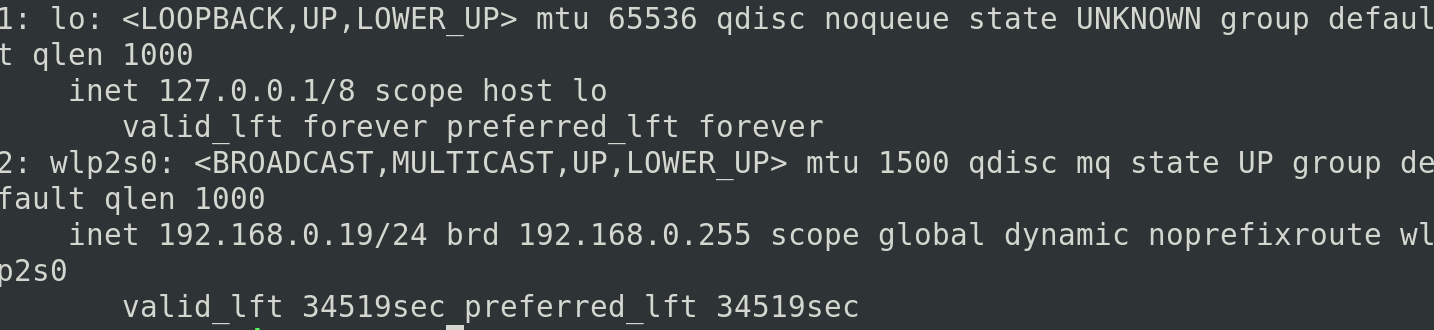
\includegraphics[width=10cm]{ressources/ip.png}
        \captionof{figure}{Adresse de la machine}
        \label{IMG}
    \end{center}
\note[item]{adresse de broadcast; adresse 169.254... = quand machine n'obtient pas adresse via DHCP, elle s'en crée une}
\note[item]{adresse 169.254... = quand machine n'obtient pas adresse via DHCP, elle s'en crée une}
\end{frame}
\section{Structure maillée}
\subsection{Les routeurs}
\begin{frame}
    \frametitle{Repérer une machine sur le réseau}

    Un réseau est structuré autour des \textbf{routeurs}.
\begin{itemize}
    \item<1-> Les routeurs d'accès
    \item<2-> Les routeurs internes
\end{itemize}

\end{frame}

\begin{frame}
    \frametitle{}

    \begin{center}
        \centering
        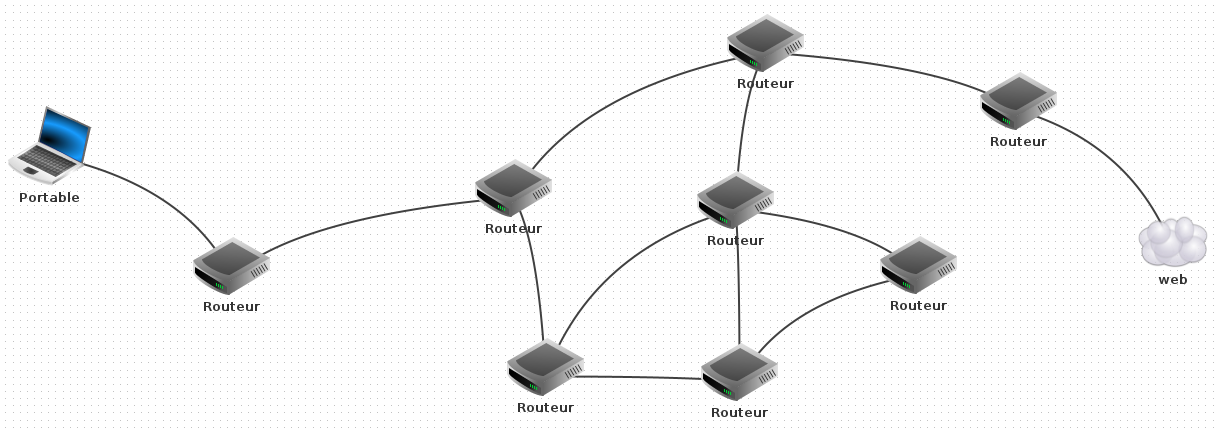
\includegraphics[width=10cm]{ressources/reseau.png}
        \captionof{figure}{Topologie d'un réseau}
        \label{reseau}
    \end{center}

\end{frame}

\begin{frame}[fragile]
    \frametitle{}

    \begin{activite}
        \begin{enumerate}
            \item Sur la figure \ref{reseau}, repérer les routeurs d'accès, les routeurs internes.
            \item Installer le paquet \emph{traceroute}
            \begin{center}
                \begin{lstlisting}[language=bash]
sudo apt install traceroute
                \end{lstlisting}
                \captionof{code}{Installation d'un paquet}
                \label{ip}
            \end{center}
            \item Taper la commande (code \ref{trace}).
            \begin{center}
                \begin{lstlisting}[language=bash]
traceroute fr.wikipedia.org
                \end{lstlisting}
                \captionof{code}{Tracer le chemin suivi vers une destination}
                \label{trace}
            \end{center}
        \end{enumerate}
        \end{activite}

\end{frame}
\begin{frame}
    \frametitle{}

    \begin{center}
        \centering
        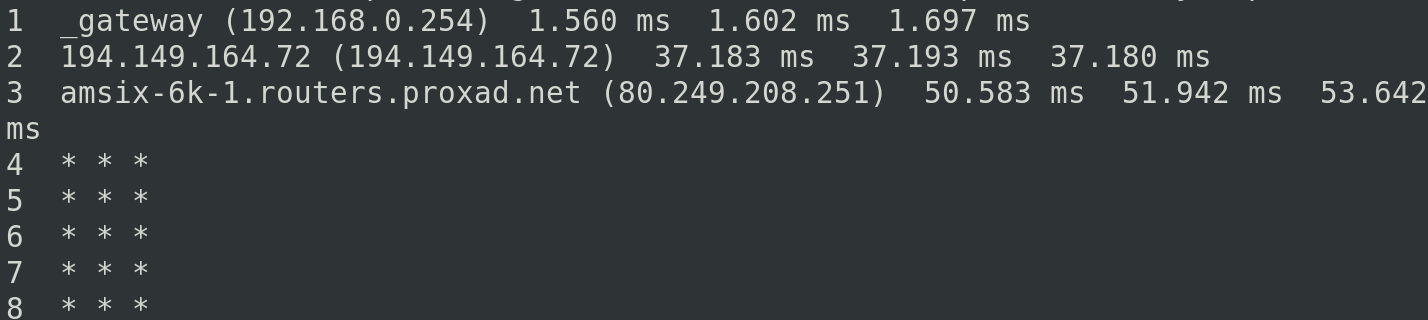
\includegraphics[width=10cm]{ressources/trace.png}
        \captionof{figure}{Traceroute}
        \label{IMG}
    \end{center}
\begin{itemize}
    \item Envoi de 3 paquets $\;\rightarrow\;$ donne une information moyenne
    \item La commande envoie des paquets avec un TTL (Time To Live) croissant pour découvrir la route au fur et à mesure.
    \item * * * ?
    \begin{itemize}
        \item La commande limite le TTL à 30
        \item les serveurs rejettent les paquets UDP
    \end{itemize} 
    \note[item]{Le serveur destinataire rejette les paquets UDP (User Datagram Protocol) (n'accepte que les TCP - Transmission Control Protocol).}

    \note[item]{L'option -I de traceroute permet d'envoyer des paquets avec le protcole ICMP (Internet Control Message Protocol) = ping}
\end{itemize}
\end{frame}
\begin{frame}[fragile]
    \frametitle{Envoi de paquet ICMP}

    \begin{center}
        \begin{lstlisting}[language=bash]
sudo traceroute -I fr.wikipedia.org        
        \end{lstlisting}
        \captionof{code}{Option de traceroute}
        \label{moncode}
    \end{center}

\end{frame}
\subsection{Adresse IP d'un routeur}
\begin{frame}
    \frametitle{Un routeur est une \textbf{passerelle} entre plusieurs réseaux.}
    
    \begin{aretenir}[]
        Un routeur possède autant d'\textbf{interfaces} que de réseaux associés.
    \end{aretenir}
\note{interface = carte réseau (filaire, wifi)}
\end{frame}

\begin{frame}
    \frametitle{}

    \begin{center}
        \centering
        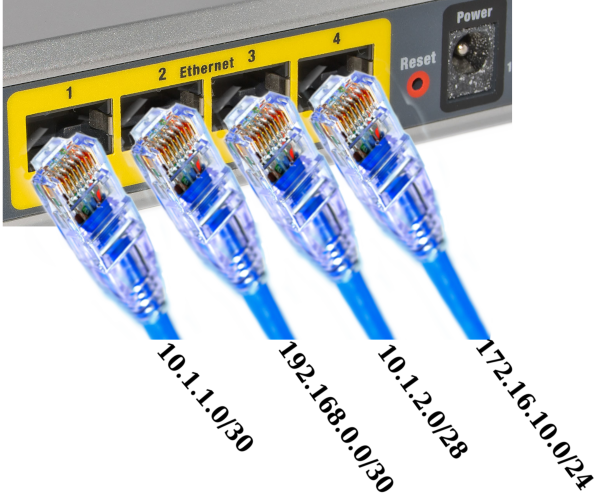
\includegraphics[width=5cm]{ressources/routeur-adresses.png}
        \captionof{figure}{Un routeur lié à quatre réseaux}
        \label{routeur}
    \end{center}
    \begin{activite}
    Le routeur en figure \ref{routeur} est associé au quatre réseaux indiqués. Donner la plus grande adresse possible à chacune des \emph{interfaces} du routeur.
    \end{activite}

\end{frame}

\begin{frame}
    \frametitle{}

    \begin{center}
        \centering
        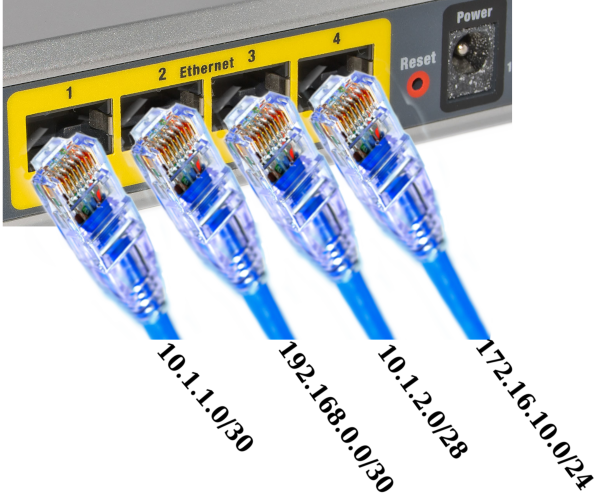
\includegraphics[width=5cm]{ressources/routeur-adresses.png}
        \captionof{figure}{Un routeur lié à quatre réseaux}
        \label{routeur}
    \end{center}
    L'adresse de broadcast (diffusion) à tous ses bits à 1. On prend alors l'avant-dernière pour le réseau.
    \begin{itemize}
        \item réseau 10.1.1.0/30 $\;\rightarrow\;$ interface 10.1.1.2
        \item réseau 192.168.0.0/30 $\;\rightarrow\;$ interface 192.168.0.2
        \item réseau 10.1.2.0/28 $\;\rightarrow\;$ interface 10.1.2.14
        \item réseau 172.16.10.0/24 $\;\rightarrow\;$ interface 172.16.10.254
    \end{itemize}
\note{$2^{32-n}$ adresses possibles et la plus grande: $2^n -1$}
\end{frame}
\subsection{La table de routage}
\begin{frame}
    \frametitle{}

    \begin{itemize}
        \item<1->Un paquet circule de \textbf{proche en proche}.
        \item <2->La table de routage indique le prochain \emph{routeur voisin}.
    \end{itemize}

\end{frame}

\begin{frame}
    \frametitle{}

    \begin{center}
        Il n'y a pas de route définie entre l'émetteur et le destinataire. On parle de \textbf{commutation par paquets}.
    \end{center}
\note[item]{Deux paquets qui partent de l'émetteur ne vont pas suivre le même chemin.}
\note[item]{Commutation de circuits = liaison physique entre émetteur et destinaire $\;\rightarrow\;$ téléphone}
\end{frame}

\begin{frame}[fragile]
    \begin{activite}
        Afficher la table de routage de la machine.
        \begin{lstlisting}[language=bash]
ip route
                \end{lstlisting}
        \end{activite}
\end{frame}
\begin{frame}
    \frametitle{}

    \begin{center}
    \centering
    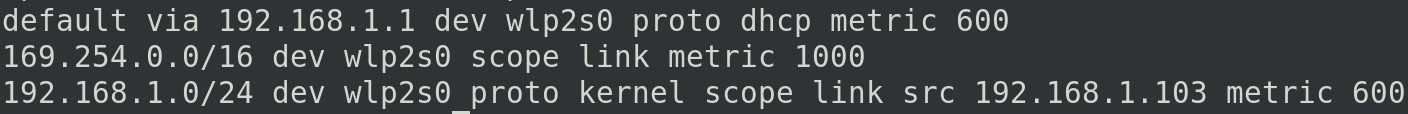
\includegraphics[width=10cm]{ressources/route.png}
    \captionof{figure}{Table de routage d'un ordinateur personnel}
    \label{IMG}
    \end{center}

\end{frame}
\end{document}